%% SW design: klassebeskrivelse devkit Controllers
\newpage

\begin{figure}[htbp] \centering
{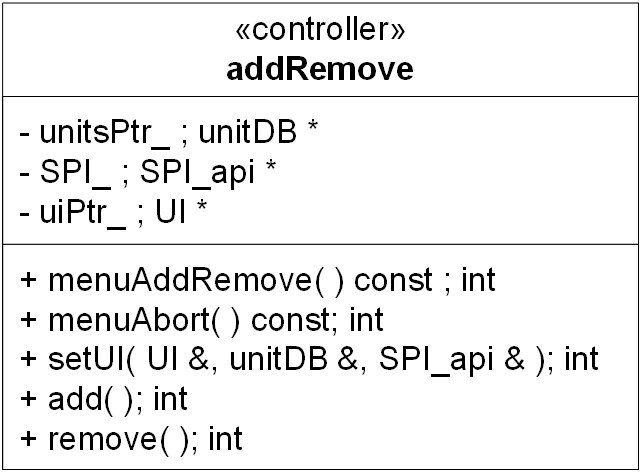
\includegraphics[scale=1.5]{filer/design/Klassediagrammer/sw_addRemove}}
\caption{Klasse addRemove}
\label{fig:addRemove klassediagram}
\end{figure} 

{\centering
\textbf{addRemove}\par
}
\textbf{Ansvar:} At styre forløbet i UC1: Tilføj / fjern enhed. \

\textbf{Attributter:}
\begin{itemize}
	\item \verb+unitDB * unitsPtr_+ Pointer til associeret objekt
	\item \verb+SPI_api * SPI_+ Pointer til associeret objekt
	\item \verb+UI * uiPtr_+ Pointer til associeret objekt
\end{itemize}

\verb+int menuAddRemove( ) const+ \\
\textbf{Parametre:} Modtager ingen parametre. \\
\textbf{Returværdi:} 0 ved succes ellers negativ i overenstemmelse med fejl-listen. \\
\textbf{Beskrivelse:} Henter opsatte Enheder fra \verb+unitDB+, tilføjer dem til tabellen i \verb+winAddRemove+-klassen og viser tilføj/fjern-brugerfladen ved at kalde \verb+showAddRemove()+-metoden i \verb+UI+-klassen.\\

\verb+int menuAbort( ) const+ \\
\textbf{Parametre:} Modtager ingen parametre. \\
\textbf{Returværdi:} 0 ved succes ellers negativ i overenstemmelse med fejl-listen. \\
\textbf{Beskrivelse:} Viser hovedmenuen ved at kalde \verb+showMain()+-metoden i \verb+UI+-klassen.\\

\verb+int setUI( UI &, unitDB &, SPI_api &) const+ \\
\textbf{Parametre:} Parametre til associerede objekter. \\
\textbf{Returværdi:} 0 ved succes ellers negativ i overenstemmelse med fejl-listen. \\
\textbf{Beskrivelse:} Gemmer parametrene i klassens private medlems-attributter. \\

\verb+int add( ) const+ \\
\textbf{Parametre:} Modtager ingen parametre. \\
\textbf{Returværdi:} 0 ved succes ellers negativ i overenstemmelse med fejl-listen. \\
\textbf{Beskrivelse:} Henter værdier fra felterne i \verb+winAddRemovePar+-vinduet. Kalder \verb+verify()+ og \verb+config()+ i \verb+SPI_api+-klassen og opdaterer enhedslisten ved at hente Enheder med \verb+getUnits()+, indskrive den nye Enhed og gemme igen med \verb+saveUnit()+. Til sidst vises Tilføj/fjern-brugerfladen igen ved at kalde \verb+menuAddRemove()+ i \verb+UI+. \\

\verb+int remove( ) const+ \\
\textbf{Parametre:} Modtager ingen parametre. \\
\textbf{Returværdi:} 0 ved succes ellers negativ i overenstemmelse med fejl-listen. \\
\textbf{Beskrivelse:} Henter den markerede Enhed fra listen i \verb+winAddRemove+-vinduet. Opdaterer enhedslisten i \verb+unitDB+ ved at hente Enheder med \verb+getUnits()+, indskriver -1 som temperatur- og fugtighedsgrænse og gemmer igen med \verb+saveUnit()+.\\

\begin{figure}[htbp] \centering
{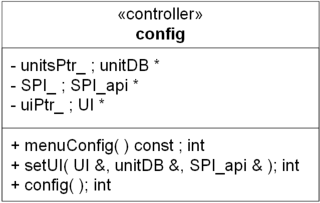
\includegraphics[scale=1.5]{filer/design/Klassediagrammer/sw_config}}
\caption{Klasse config}
\label{fig:config klassediagram}
\end{figure} 

{\centering
\textbf{Config}\par
}
\textbf{Ansvar:} At styre forløbet i UC2: Konfig. \

\textbf{Attributter:}
\begin{itemize}
	\item \verb+unitDB * unitsPtr_+ Pointer til associeret objekt
	\item \verb+SPI_api * SPI_+ Pointer til associeret objekt
	\item \verb+UI * uiPtr_+ Pointer til associeret objekt
\end{itemize}

\verb+int menuConfig( ) const+ \\
\textbf{Parametre:} Modtager ingen parametre. \\
\textbf{Returværdi:} 0 ved succes ellers negativ i overenstemmelse med fejl-listen. \\
\textbf{Beskrivelse:} Opdaterer tabellen i \verb+winConfig+-vinduet med opsatte Enheder, ved at hente dem fra \verb+unitDB+ med \verb+getUnits()+. Viser til sidst Konfigurer-brugerfladen ved at kalde \verb+showConfig()+ i \verb+UI+.\\

\verb+int setUI( UI &, unitDB &, SPI_api &) const+ \\
\textbf{Parametre:} Parametre til associerede objekter. \\
\textbf{Returværdi:} 0 ved succes ellers negativ i overenstemmelse med fejl-listen. \\
\textbf{Beskrivelse:} Gemmer parametrene i klassens private medlems-attributter. \\

\verb+int config( ) const+ \\
\textbf{Parametre:} Modtager ingen parametre. \\
\textbf{Returværdi:} 0 ved succes ellers negativ i overenstemmelse med fejl-listen. \\
\textbf{Beskrivelse:} Henter værdier fra felterne i \verb+winConfigPar+-vinduet samt tabellen i \verb+winConfig+. Henter den markerede række fra tabellen og opdaterer parametrene ud fra felterne. Kalder \verb+config()+ i \verb+SPI_api+ med værdierne for at konfigurerer Enheden. Til sidst opdateres enhedsdatabasen, \verb+unitDB+, ved at hente enhederne med \verb+getUnits()+, opdaterer de aktuelle punkter, og gemme det igen med \verb+saveUnit()+ og brugerfalden opdateres ved at kalde \verb+menuConfig+. \\

\begin{figure}[htbp] \centering
{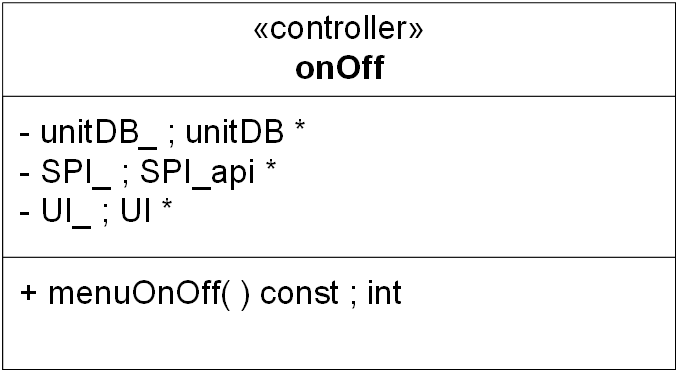
\includegraphics[scale=1.5]{filer/design/Klassediagrammer/sw_onOff}}
\caption{Klasse onOff}
\label{fig:onOff klassediagram}
\end{figure} 

{\centering
\textbf{onOff}\par
}
\textbf{Ansvar:} At styre forløbet i UC3: Aktiver / deaktiver. \

\textbf{Attributter:}
\begin{itemize}
	\item \verb+unitDB * unitsPtr_+ Pointer til associeret objekt
	\item \verb+SPI_api * SPI_+ Pointer til associeret objekt
	\item \verb+UI * uiPtr_+ Pointer til associeret objekt
\end{itemize}

\verb+int menuOnOff( ) const+ \\
\textbf{Parametre:} Modtager ingen parametre. \\
\textbf{Returværdi:} 0 ved succes ellers negativ i overenstemmelse med fejl-listen. \\
\textbf{Beskrivelse:} Fylder listen fra \verb+winOnOff+-vinduet med data fra enhedslisten, \verb+unitDB+, med \verb+getUnits()+ og viser Aktiver/deaktiver-brugerfladen ved at kalde \verb+showOnOff()+-metoden i \verb+UI+. \\

\verb+int menuAbort( ) const+ \\
\textbf{Parametre:} Modtager ingen parametre. \\
\textbf{Returværdi:} 0 ved succes ellers negativ i overenstemmelse med fejl-listen. \\
\textbf{Beskrivelse:} Viser hovedmenuen ved at kalde \verb+showMain()+-metoden i \verb+UI+-klassen.\\

\verb+int On( ) const+ \\
\textbf{Parametre:} Modtager ingen parametre. \\
\textbf{Returværdi:} 0 ved succes ellers negativ i overenstemmelse med fejl-listen. \\
\textbf{Beskrivelse:} Henter markerede Enhed fra listen i \verb+winOnOff+-vinduet og aktiverer denne ved at kalde \verb+activate()+ i \verb+SPI_api+. Her efter opdateres enhedslisten, \verb+unitDB+, ved at hente Enhederne med \verb+getUnits()+ og gemme dem igen med \verb+saveUnit()+. Listen i vinduet opdateres også ved at skrive \verb+[Aktiv]+ efter enhedens navn. \\

\verb+int Off( ) const+ \\
\textbf{Parametre:} Modtager ingen parametre. \\
\textbf{Returværdi:} 0 ved succes ellers negativ i overenstemmelse med fejl-listen. \\
\textbf{Beskrivelse:} Henter markerede Enhed fra listen i \verb+winOnOff+-vinduet og deaktiverer denne ved at kalde \verb+deactivate()+ i \verb+SPI_api+. Her efter opdateres enhedslisten, \verb+unitDB+, ved at hente Enhederne med \verb+getUnits()+ og gemme dem igen med \verb+saveUnit()+. Listen i vinduet opdateres også ved at skrive \verb+[Deaktiv]+ efter enhedens navn. \\

\verb+int setUI( UI &, unitDB &, SPI_api &) const+ \\
\textbf{Parametre:} Parametre til associerede objekter. \\
\textbf{Returværdi:} 0 ved succes ellers negativ i overenstemmelse med fejl-listen. \\
\textbf{Beskrivelse:} Gemmer parametrene i klassens private medlems-attributter. \\

\begin{figure}[htbp] \centering
{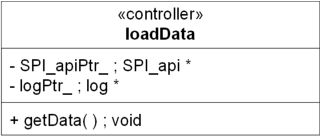
\includegraphics[scale=1.5]{filer/design/Klassediagrammer/sw_loadData}}
\caption{Klasse loadData}
\label{fig:loadData klassediagram}
\end{figure} 

{\centering
\textbf{loadData}\par
}
\textbf{Ansvar:} At styre forløbet i UC4: Databehandling. \

\textbf{Attributter:}
\begin{itemize}
	\item \verb+SPI_api * SPI_apiPtr_+ Pointer til associeret objekt
	\item \verb+log * logPtr_+ Pointer til associeret objekt
\end{itemize}

\verb+loadData( SPI_api *, log *, QObject * = 0)+ \\
\textbf{Parametre:} Parametre til associerede objekter. \verb+QObject+ bruges ikke, men er nødvendig da klassen arver fra \verb+QObject+-klassen. \\
\textbf{Returværdi:} Ingen. \\
\textbf{Beskrivelse:} Opretter og starter en \verb+QTimer+ samt opsætter en forbindelse mellem timerens udløbs-event og metoden \verb+getData()+. \\

\verb+void getData( )+ \\
\textbf{Parametre:} Modtager ingen parametre \\
\textbf{Returværdi:} 0 ved succes ellers negativ i overenstemmelse med fejl-listen \\
\textbf{Beskrivelse:} Henter log-data ved at kalde \verb+getLog()+ i \verb+SPI_api+. Hvis denne indeholder måleinformation fra sensorerne gemmes disse iht. dataprotokollen, \ref{header:dataprotokol} med et kald til \verb+saveLog()+ i \verb+log+. Bemærk at der skal konverteres mellem \verb+QVector+ og \verb+std::vector+ som resultat af at \verb+SPI_api+ ikke er skrevet i Qt frameworket.\\

\begin{figure}[htbp] \centering
{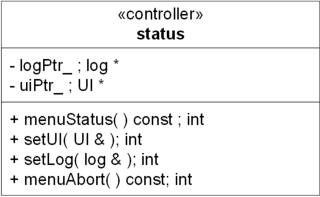
\includegraphics[scale=1.5]{filer/design/Klassediagrammer/sw_status}}
\caption{Klasse status}
\label{fig:status klassediagram}
\end{figure} 

{\centering
\textbf{status}\par
}
\textbf{Ansvar:} At styre forløbet i UC5: Tjek status. \

\textbf{Attributter:}
\begin{itemize}
	\item \verb+log * logPtr_+ Pointer til associeret objekt
	\item \verb+UI * uiPtr_+ Pointer til associeret objekt
\end{itemize}

\verb+int menuStatus( ) const+ \\
\textbf{Parametre:} Modtager ingen parametre. \\
\textbf{Returværdi:} 0 ved succes ellers negativ i overenstemmelse med fejl-listen. \\
\textbf{Beskrivelse:} Henter seneste data-logning med \verb+latest()+ i \verb+log+, gemmer dataene i felterne i \verb+winStatus+-vinduet og aktiverer felterne, hvis der er data. Hvis der ikke er data deaktiveres felterne blot. Her efter vises Vis Status-brugerfladen ved at kalde \verb+showStatus+ i \verb+UI+.\\

\verb+int setUI( UI & ) const+ \\
\textbf{Parametre:} Parameter til associeret objekt. \\
\textbf{Returværdi:} 0 ved succes ellers negativ i overenstemmelse med fejl-listen. \\
\textbf{Beskrivelse:} Gemmer parameter i klassens private medlems-attribut. \\

\verb+int setLog( log & ) const+ \\
\textbf{Parametre:} Parameter til associeret objekt. \\
\textbf{Returværdi:} 0 ved succes ellers negativ i overenstemmelse med fejl-listen. \\
\textbf{Beskrivelse:} Gemmer parameter i klassens private medlems-attribut. \\

\verb+int menuAbort( ) const+ \\
\textbf{Parametre:} Modtager ingen parametre. \\
\textbf{Returværdi:} 0 ved succes ellers negativ i overenstemmelse med fejl-listen. \\
\textbf{Beskrivelse:} Viser hovedmenuen ved at kalde \verb+showMain()+-metoden i \verb+UI+-klassen.\\

\begin{figure}[htbp] \centering
{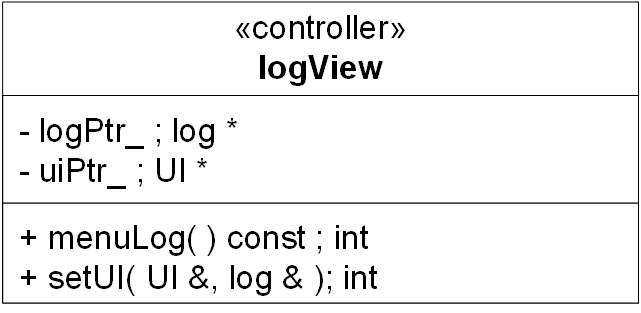
\includegraphics[scale=1.5]{filer/design/Klassediagrammer/sw_logView}}
\caption{Klasse logView}
\label{fig:logView klassediagram}
\end{figure}

{\centering
\textbf{logView}\par
}
\textbf{Ansvar:} At styre forløbet i UC6: Udskriv log. \

\textbf{Attributter:}
\begin{itemize}
	\item \verb+log * logPtr_+ Pointer til associeret objekt
	\item \verb+UI * uiPtr_+ Pointer til associeret objekt
\end{itemize}

\verb+int menuLog( ) const+ \\
\textbf{Parametre:} Modtager ingen parametre. \\
\textbf{Returværdi:} 0 ved succes ellers negativ i overenstemmelse med fejl-listen. \\
\textbf{Beskrivelse:} Fylder tabellen fra \verb+winLog+-vinduet med data fra loggen ved at hente denne med \verb+getLog()+ i \verb+log+. Viser Log-brugerfladen ved at kalde \verb+showLog()+ i \verb+UI+.\\

\verb+int setUI( UI &, log & ) const+ \\
\textbf{Parametre:} Parametre til associerede objekter. \\
\textbf{Returværdi:} 0 ved succes ellers negativ i overenstemmelse med fejl-listen. \\
\textbf{Beskrivelse:} Gemmer parametrene i klassens private medlems-attributter. \\
